\documentclass[12pt]{article}

\usepackage{pgfplots}
\pgfplotsset{width=10cm, compat=1.9}
\usepgfplotslibrary{external}
%\tkzexternalize

\usepackage{mathtools}

\usepackage{blindtext}

\usepackage{graphicx}

\usepackage{float}

\usepackage{listings}

\usepackage{color}
 
\definecolor{codegreen}{rgb}{0,0.6,0}
\definecolor{codegray}{rgb}{0.5,0.5,0.5}
\definecolor{codepurple}{rgb}{0.58,0,0.82}
\definecolor{backcolour}{rgb}{1,1,1}
 
\lstdefinestyle{mystyle}{
  backgroundcolor=\color{backcolour},
  commentstyle=\color{codegreen},
  keywordstyle=\color{magenta},
  numberstyle=\tiny\color{codegray},
  stringstyle=\color{codepurple},
  basicstyle=\footnotesize,
  breakatwhitespace=false,
  breaklines=true,
  captionpos=b,
  keepspaces=true,
  numbers=left,
  numbersep=5pt,
  showspaces=false,
  showstringspaces=false,
  showtabs=false,
  tabsize=2
}
 
\lstset{style=mystyle}

\usepackage[backend=biber, style=authoryear]{biblatex}
\addbibresource{bibliography.bib}

\title{Efficiency Per Marginal Intermediary Node in a Simple Artificial Neural Network}
\author{Abdullah Binladin}
\date{April 2019}

\begin{document}
\maketitle

\tableofcontents
\pagebreak

\section{Research Methods and Objectives}

\subsection{Justification\label{history}}

It is no secret that Artificial Intelligence is among the most prominent fields of Computer Science today. It is also no secret that big media and tech
companies collect your browsing data to train AI (Artificial Intelligence) algorithms to serve various purposes (usually to personalize advertisements to you, the user). For instance, Netflix uses your viewing history to train an AI to predict what movie or T.V. Series you may be interested in watching next.

An arguably more nefarious example may be in the case of the two online marketing giants, Facebook and Google. At the forefront of A.I. research, Facebook and Google are known to log their users browsing history to use or sell it as training data for Artificial Intelligence Algorithms. The A.I in question is then used to display advertisements to the user that the AI predicts the user would be likely to click on. Both firms have been criticized for their allegedly morally dubious business practices regarding how they respect their users' right to privacy. In 2018, Facebook CEO Mark Zuckerberg was required to explain to the U.S. Congress how precisely facebook used their user's data. The interview was broadcast live and lasted an entire eight hours.

While the exact artificial neural network algorithm any given media or tech company uses is an extremely closely guarded trade secret - the tech equivalent of Coca Cola's recipe- They all generally the same abstract subcomponents, like how all sodas are some combination of fizzy water, flavouring and colour.

As artificial intelligence is so pervasive in the modern world, it is then relevant to understand how it is that AI algorithms are built and how they function. Thus, this paper assumes that the reader is comfortable with multivariate calculus and is somewhat familiar with linear algebra.

\subsection{Objectives \label{objectives}}

The objective of this research experiment is to model the relationship between the efficiency of a Simple Artificial Neural Network and the number of neurons in its intermediate hidden layer and, if it is possible, to find the optimal number of neurons for this experiment.

As the network used will be a simple artificial neural network, the neural network in this experiment will only have three layers of neurons:

\begin{itemize}
  \item An input layer of two nodes
  \item A single hidden intermediate layer of variable size
  \item An output layer of a single node
\end{itemize}

The neural network will attempt to predict the expected output of a logical XOR (exclusive OR) gate. An XOR gate is defined as such: an output is true if and only if either of the inputs is true. See Figure \ref{xortable} for a truth table. As a boolean algebraic expression, it is defined as in Equation 1.

\begin{equation}
  \textrm{A XOR B}: A \wedge B \vee \neg(A \wedge B)
\end{equation}


I am uncertain as to how an additional node in the hidden layer will affect computational runtime speed. I expect that no matter the number of nodes, the runtime will increase at a factor of $O(n^2)$ such that $n$ is the number of neurons in the intermediate layer. It is also plausible that it could be some form of $O(nlog(n))$. Admittedly I am stretching the definition of Bachmann-Landau notation but it adequately conveys my expectations for the experiment.

\begin{figure}[h]
  \begin{center}
  \begin{tabular}{|c|c|c|}
  \hline
  \multicolumn{3}{|c|}{XOR Gate} \\
  \hline
  Input 1 & Input 2 & Output \\
  \hline
  0 & 0 & 0 \\
  1 & 0 & 1 \\
  0 & 1 & 1 \\
  1 & 1 & 0 \\
  \hline
  \end{tabular}
  \end{center}
  \caption{An XOR gate in table format \label{xortable}}
\end{figure}

\subsection{Methods \label{methods}}

\begin{figure}
  \begin{center}
  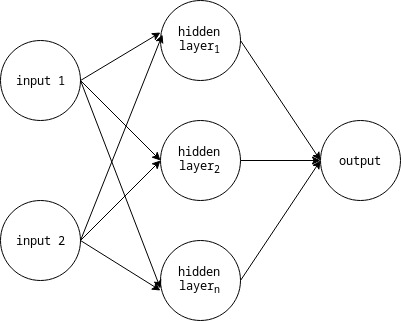
\includegraphics[width=0.7\textwidth]{ANN-diagram.jpg}
  \caption{Model of a simple artificial neural network with a hidden layer of length \(n\)\label{anndiagram}}
  \end{center}
\end{figure}

Each neuron in the input layer will represent either of the possible inputs of the XOR gate. The output layer will have one neuron containing a number between 0 and 1. This number represents the neural network's certainty level.

\begin{itemize}
  \item The more certain the neural network is that the output should be 1, the closer the output neuron will be to 1
  \item The more certain the neural network is that the output should be 0, the closer the output neuron will be to 0
\end{itemize}

The research experiment will be run in a Python 3.7.3 script as Python is both easy to read and is the industry standard for A.I. development. The simple neural network can be modeled as described in Figure \ref{anndiagram}. The arrows represent the synaptic weights between nodes; \begin{math}n\end{math} indicates the real coordinate space the intermediate vector lies in.

The python algorithm for building the artificial neural network can be found in \ref{neuralnetpy}. Upon attempting the experiment I quickly realized that the neural network generated too much data to organize by hand, so I wrote DataCollector.py (Section \ref{datacollectorpy})to store and organize the results of the experiment.

Each layer is written as an array of neurons, and each neuron has a corresponding array of synaptic weights. Python does not natively support arrays; instead, it utilizes (Linked) Lists as its main method for aggregating data. Instead, I will be using the numpy Python package.

The independent variable will be the length of the hidden layer. I will begin with a hidden layer of length 1 and increment its length by 1 in each stage of the experiment, up to a final value n.

The dependent variable will be how certain the neural network is of its predicted output. The output neuron denoted by \({Y_o}\) will contain a value such that \(0 < Y_o < 1\); This will correspond to the actual output of an XOR gate, which is either 0 or 1. The closer the output of the neural network is to either 1 or 0, the more certain the neural network is that its output is correct. It should be mentioned that because each neuron is passed through the sigmoid function \(\sigma(x)\) (As described in section \ref{neuron}), the predicted output will never be equal to 1 or 0; thus it will never be fully certain.

The control variables will be the number of times the neural network is trained, and the number of neurons in the intermediate hidden layer. The former is crucial because the more often a neural network is trained, the more accurate the output becomes. It is only logical, then, to conclude that a change in the number of times a neural network is trained will skew the results of the experiment. The latter's significance is similar; The objective of this experiment is to analyze the effect of an additional neuron on the efficiency of the algorithm- any additional layers would muddy an individual neurons effect on the final predicted output.

All of the data collected is quantitative- there's no qualitative data to collect.

% Talk about the specifics of the neural network (no stochastic Backprop, no optimized init, vanilla barebones NN, etc. )

The neural network will be a very basic, barebones, 'vanilla' algorithm; I will not be using any form of deep learning implementations, no optimized initialization of synaptic weights and biases, and the gradient descent algorithm will not be stochastic.

\section{Literature Review}

\subsection{Definition of an Artificial Neural Network \label{ANN-definition}}

An artificial neural network is a mathematical model loosely based off of how the human brain works. The concept is as follows: a set of layers of neurons are interlinked via synapses. If a neuron is close to being 'correct', the synapse it's connected to 'fires' and the synaptic weight between them is strengthened. While the latest developments in A.I. have allowed for more complex and more accurate initializations of neurons and synaptic weights, the standard method is to assign each neuron and synaptic weight some random floating-point value between 0 and 1.

An artificial neural network algorithm is created via two processes: building and training \textcite{GCPGreyAI}. The building process does the actual strengthening or weakening of the synaptic weights between neurons. The training process calculates the error and the correction. These two processes are then run sequentially many hundreds or thousands of times, causing the algorithm to become a little more accurate each iteration.

At no point does either the human, the training processor or the building processor understand precisely what the artificial neural network algorithm actually is or how it arrives at its conclusions; only that with each iteration of training and building, the algorithm becomes marginally more accurate. It is as nebulous and abstract as it sounds.

\subsection{Neurons/Nodes \label{neuron}}

As \textcite{DeepLearningCh1} says, a \textit{neuron} (also known as a \textit{node})is simply an element of an array (or a component of a vector, from a mathematical perspective). It contains a floating-point number between 0 and 1. This number is called the neuron's \textit{activiation}. It is this number that represents how 'correct' a neuron is, as is referred to in section \ref{ANN-definition}. Each neuron is connected to every neuron in the adjacent layer via synaptic weights.

To calculate the value of a neuron, a linear combination is taken of each connected neuron $z$ of the preceding layer $l$ and its corresponding weight \textcite{sharma2017}. In other words, its value is the dot product of each of those neuron layers and their weight matricies:

\begin{equation} \label{forwardpropequation}
  z = \sum_{i=1}^{n}(z^{(L-1)} \cdot w_{jk})
\end{equation}

%s Talk about activation functions here
However, this results in a value of \begin{math} -\infty < Y < \infty \end{math}. This, however, does not fit our model for a neuron. There is no upper or lower limit, so we can't calculate how activated a given neuron \(Y\) is- there is no frame of reference. Thus, it is necessary to 'squeeze' the value of \(Y\) into some value between 0 and 1. This is achieved by passing it into what is called the \textit{Activation function}.\textcite{sharma2017}.

There are many activation functions that exist. Some examples are the \(RelU(x)\) function and the \(tanh\) function. For the purpose of this experiment I will be using the sigmoid function, also known as the logistic function. It is the classic neural network \textcite{DeepLearningCh2} defined as in Equation \ref{sigmoid}:

\begin{equation} \label{sigmoid}
  Y = \sigma(z) = \frac{1}{1 + e ^ {-z}}
\end{equation}

% Talk a bit about the history of the sigmoid function in AI, also insert sigmoid graph

As can be seen in Figure \ref{sigmoidgraph}, the graph of the sigmoid function has two horizontal asymptotes: one at \(y = 1\) and one at \(y = 0\), which also fits conveniently with our training goals. No matter what value $z$ is, \(\sigma(Y)\) will always be between 1 and 0.

\begin{figure}[h]
  \centering
  \begin{tikzpicture}
  \begin{axis}[
  axis lines = left,
  xlabel = $Y$,
  ylabel = $\sigma (Y)$
  ]
  \addplot [
  domain = -10:10,
  samples = 100,
  color = blue,
  ] {1 / (1 + e^-x)};

  \end{axis}
  \end{tikzpicture}
  \caption{Graph of $\sigma(Y)$} \label{sigmoidgraph}
\end{figure}

\subsection{Synaptic Weights \label{weights}}

A \textit{Synaptic Weight} is a ratio representing the strength of the connection between any two neurons \textcite{shamdasani2017}. As shown in Figure \ref{anndiagram}, every neuron in any given layer is connected to every single other neuron in the layer preceding it. In terms of Computer Science, a set of synaptic weights is functionally identical to a layer of neurons- it is treated as a vector of floating point numbers. The only major difference is that no activation function is applied to a synaptic weight.

The synaptic weights are the main driving force behind an artificial neural network algorithm. With each iteration of the building/training cycle, the synaptic weight is adjusted depending on the severity of the error of that cycle. The more 'incorrect' a synaptic weight is, the more it is adjusted in a given cycle.

\subsection{Layers}

In section \ref{neuron}, I referred to a neuron being an element of an array. In the context of artificial neural networks, this array comes in the form of a \textit{layer}. An artificial neural network is essentially a collection of neurons linked via synaptic weights. The neurons are organized into one of three different categories of neurons. These categories are in the form of layers. These categories are:

\begin{itemize}
  \item The input layer
  \item The hidden intermediate layer(s)
  \item The output layer
\end{itemize}

All neurons in all three layers are structurally identical- a neuron is simply a variable that holds a floating-point number between 0 and 1. The difference is in what they do: The neurons in the input layer are immutable as it they contain the values of the input, the intermediary hidden layer contains neurons whose values are constantly adjusting and rebalancing depending on the output of the algorithm and the application of gradient descent, and the output layer simply contains the predicted output of a neural network after a training cycle

\subsubsection{A Note on Deep Learning}

\begin{figure}[h]
  \centering
  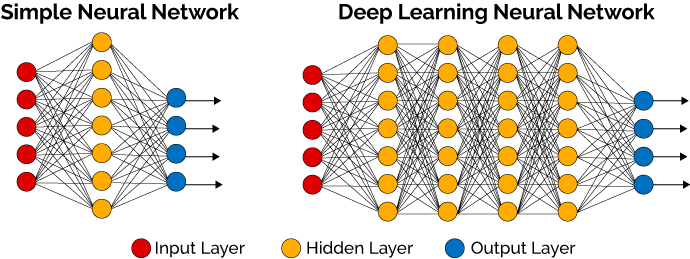
\includegraphics[width=\textwidth]{DeepLearning-diagram.png}
  \caption{A contrast between a simple neural network vs a deep learning neural network. Courtesy of \textcite{vazquez17}. \label{deeplearningfig}}
\end{figure}

If you have kept up with Artificial Intelligence on the news over the last decade, you may have heard of \textit{Deep Learning} algorithms a number of years ago. Having risen in popularity early this decade, Deep Learning is a relatively new field in Machine Learning where the hidden layer is many layers deep (hence the name), with the intent to emulate the neocortex of the human brain \textcite{Hof2013}. In other words, in a deep learning algorithm the hidden layer is a matrix of neurons, rather than a vector.

One of the pitfalls of deep learning algorithms is that because there are so many neurons subdivided into many hidden intermediary layers that it's almost impossible for any human to grasp the effect of any one neuron (or even a collection of neurons) on the overall output of the neural network. This is covered in more depth in Section \ref{backprop}.

Deep learning, along with \textit{Generated Adversarial Networls} is currently at the forefront of A.I. Research; It is currently used for all kinds of tasks, from image classification tasks to virtual assistants such as \textit{Google Now} and Amazon's \textit{Alexa}. \textcite{vazquez17}. The most complex deep learning algorithms can identify objects in an image almost as well as a human can.

\subsection{Forward Propogation \label{foreprop}}

The 'training' and 'building' process as described in section \ref{ANN-definition} have technical definitions: Forward Propagation and Backpropagation. \textit{Forward Propagation} is the technical definition for the building process.

Forward propagation works as follows: for each neuron \(Y\) in a given layer, take the dot product of each neuron the in the previous layer and the synapse associating it with \(Y\). Equation \ref{forwardpropequation} in section \ref{neuron} models this process. This is the process that adjusts the values of the neurons of the neural network; the synapses and biases are left untouched in this stage.

\subsubsection{Bias for Inactivity}
For some tasks, it would be prudent to add some \textit{bias} variable \(b\) to the forward propagation function. This bias variable adds a bias to the algorithm by setting some minimum requirement for a neuron to activate, such that a neuron only activates of the weighted sum is greater than the bias. A bias variable can be added to a forward propagation functions as follows:

\begin{equation} \label{biasequation}
  \sum_{i=1}^{n}(\vec Y_{l-1} \cdot w_{ji}) -b
\end{equation}

As discussed before, each neuron is connected to every neuron from the previous layer, with each synapse's strength is weighted by some factor between 0 and 1. As described in equation \ref{biasequation} above, if a bias is to be added then each neuron would contain a single bias that would shift the activation function down by the size of the bias.


\subsection{Gradient Descent \label{gradient-descent}}

In order for a neural network to learn, some form of feedback algorithm must be integrated into the training process - some method for the neural network to understand how to adjust its neurons and synapses in order to improve its accuracy each training cycle.

As as stated in section \ref{ANN-definition}, the neurons and synapses are initialized randomly. Logically, you would conclude that the output of the neural network using the initial permutation of neuron and synapse values would lead to a meaningless output neuron. In the context of our experiment and objectives, our neural network could output anything from 0.999 to 0.453. Thus, it is crucial to figure out a method to somehow pare down the error each training cycle.

To calculate the margin of error of the network's output, we can take the square difference between the neural network's output \(Y_o\) and the expected output \(o\). This is called the sum squared loss function. It is defined as in Equation \ref{loss-equation}.

\begin{equation} \label{loss-equation}
  E(o , Y_o) = \sum (o - Y_o)^2
\end{equation}

This is effective as larger discrepancies between the $Y_o$ and $o$ will lead to larger corrections to the synaptic weights of the algorithm and vice-versa. Typically, the formula would sum and take the average of all of the neurons in the output layer, however since in our experiment we only have one neuron, the summation evaluates to $E(o , Y_o) = (o - Y_o)^2$, so it can be disregarded for this experiment.

\begin{figure}[h]
  \centering
  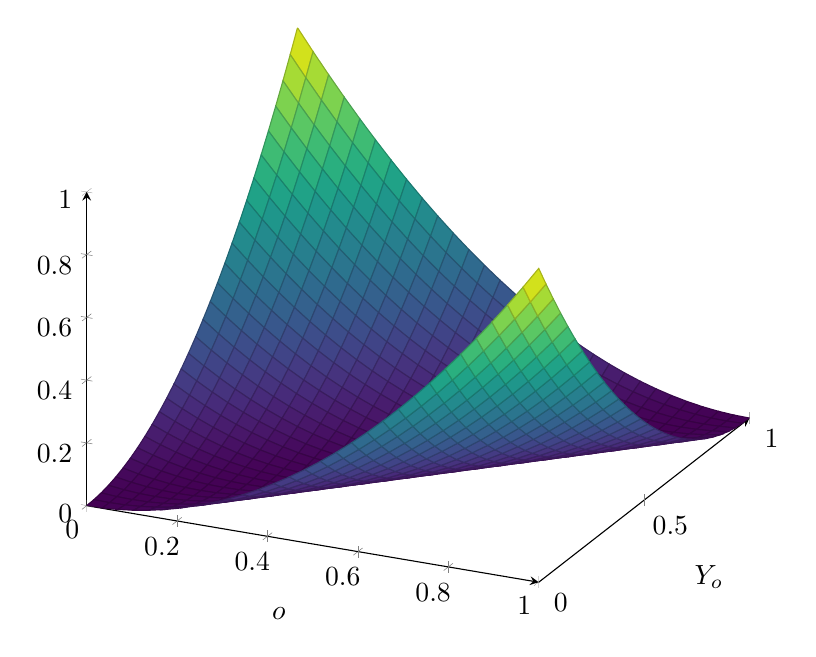
\begin{tikzpicture}
  \begin{axis}[
  colormap/viridis,
  axis lines = left,
  xlabel = $o$,
  ylabel = $Y_o$,
  ]
  \addplot3[
  surf,
  samples=30,
  domain=0:1
  ]
  {(x-y)^2};

  \end{axis}
  \end{tikzpicture}
  \caption{Graph of $E(o, Y_o)$ \label{errorgraph}}
\end{figure}

For instance, imagine that $o - Y_o = 0.9$. In that case, the synaptic weights that lead the neural network to a certain conclusion would be very incorrect. Squaring 0.9 gives a final value of 0.81, which is a very large change as it instructs the synaptic weights to shift towards the correct value $o$ by 81\%.

Contrast that with the case that $o - Y_o = 0.1$, In that case the neural network would be very close to being correct. Squaring 0.1 gives 0.01, which is a very small change as the synaptic weight shifts towards the correct value $o$ by only 1\%.

As stated in section \ref{ANN-definition}, the objective of each training cycle is for the neural network algorithm to become a little more accurate in each training cycle. Equation \ref{loss-equation} describes the error of the output of any given training cycle. Thus, we need to find the minima of Equation \ref{loss-equation}.

To visualize finding the minima of a multivariate function, imagine trying to go as low as possible a point on the plane described by the function. The First Derivative Test suggests that for any function $f(x)$ its extrema can be found in the set $\frac{df}{dx} = 0$.

In the case of \(E(o, Y_o)\) in this experiment, the variable $o$ can only ever be one of two values: 0 or 1. This is because $o$ represents the output of an XOR gate (as defined in section \ref{objectives}). Thus, we can treat it as a constant that represents either 0 or 1.

You can visualize this by 'mentally rotating' Figure \ref{errorgraph} such that you are looking at it from a 'side on' perspective, such that the parabolic shape is perpendicular to your point of view- then taking the derivative of that '2-dimensional' curve.

With that in mind, we can find the minima of $E(o, Y_o)$ by taking its partial derivative with respect to $Y_o$ - the variable that will adjust with each training cycle - and setting that to be equal to zero. This is shown in Equation \ref{loss-equation-derivative}.

\begin{equation} \label{loss-equation-derivative}
  \frac{\partial E}{\partial Y_o} = 2 (Y_o - o)
\end{equation}

Thus, by setting $\frac{\partial E}{\partial Y_o} = 0$ we can find the minima of $E(o, Y_o)$.

This technique is known as \textit{Gradient Descent}. By knowing in which direction to alter the synapses, the neural network algorithm can improve its accuracy with each training cycle.

\subsection{Backpropagation \label{backprop}}

% Insert text about brackprop
\textit{Backpropogation} is a submethod of the gradient descent algorithm, in which the weights and biases of a neural netowrk are actually adjusted. It is the step that delivers feedback into the neural network, and the process through which the neural network learns. While some may prefer the 'black box' approach to implementing the hidden layer- in which the algorithms are applied to the neural network without worrying about the small details- it is worth covering as understanding how the neural network backpropogates grants the programmer an insight into the inner workings of the algorithm, despite not fully grasping how the network interprets the values of the neurons to arrive at its conclusion as stated in Section \ref{ANN-definition}. Note that this analysis is only applicable in simpler neural networks. The deeper the intemediary hidden layers are, the more opaque the neural network becomes to the programmer.

As stated in section \ref{weights}, The synaptic weights represent the strengths of the connections between some neuron $Y$ and every neuron in the preceding layer. In other words, each $Y$ in some layer $l$ corresponds to some weight vector $\vec w$, whose components represent the strength of the link between $Y$ and every neuron in layer $l-1$.

Another thing to keep in mind when I say that $\vec w$ is a vector, I mean that in the computer science interpretation of a vector, not the physics interpretation. Consider $\vec{w}$ not as an arrow in some coordinate space $R^n$, but as an array; or an ordered list of numbers. At first glance, you would not be entirely incorrect in thinking this distinction is meaningless in the context of this experiment. As seen in Figure \ref{anndiagram}, Any neuron will only ever have a maximum of three synaptic weights connected to it, which is perfectly visualizable in a two-dimensional or three-dimensional space. However, this approach will not hold up in larger neural networks, or even this same one with a larger intermediate layer. As \textcite{DeepLearningCh3} says, it would be more easily visualizable if the magnitude of each component in $\vec w$ represents how sensitive $E(o, Y_o)$ is to each weight.

Equation \ref{biasequation} describes the factors that affect the activation of any given neuron $Y$ in layer $l$:

\begin{itemize}
  \item the bias of the neuron $Y$
  \item the weight vector $\vec{w}$, whose components represent a synaptic link between $Y$ and each neuron in $l - 1$
  \item the activation of each neuron in $l - 1$
\end{itemize}

The neurons in $l - 1$ with the highest activations have the greatest impact on the activation of $Y$, because as observed in Equation \ref{forwardpropequation} and Equation \ref{biasequation}, the activation of a neuron is calculated by taking the dot product of a neuron and its corresponding weight vector.

Neuropsychologist Donald Hebb once stated that "Neurons that fire together, wire together". The Hebbian theory of learning suggests that the more some process is repeated, the better the brain becomes at doing it. From his book, \textit{The Organization of Behaviour}:

\begin{quote}
  ``Let us assume that the persistence or repetition of a reverberatory activity (or "trace") tends to induce lasting cellular changes that add to its stability. ... When an axon of cell A is near enough to excite a cell B and repeatedly or persistently takes part in firing it, some growth process or metabolic change takes place in one or both cells such that A's efficiency, as one of the cells firing B, is increased." - \textcite{Hebb1949}
\end{quote}

It is by this process that backpropagation is inspired by. While it is true that more modern advancements in neuroscience have shown that artificial neural networks work far less similarly to how our brains actually work than we initially believed, it still stands as a well defined objective for backpropagation.

With that in mind, an individual weight $w$ also functions as a physics vector; despite only having one component, it is not a scalar; its values sign indicates in which \textit{direction} a neural network should descend $E(o, Y_o)$, and its magnitude suggests by \textit{how much} to move it in that direction per training cycle.

This is where this concept of backwards propagation fits in; by calculating the error of the output layer, we can figure out how to adjust the weights of the previous layer. And it doesn't stop there; this method is applied recursively for each neuron in layer $l$ with respect to any set of weights and neurons in layer $l - 1$, like a wave from a ripple \textit{propogating backwards} through the neural network. \textcite{Nielsen2015}.

% May integrate this into the above section EDIT: done

In the context of our research experiment, consider the activation of the output neuron $a_k^{(L)}$ (previously denoted as $o$) in the output layer $L$, such that $a_j^{(L)}$ is neuron $j$ of layer L. Equation \ref{loss-equation} in Section \ref{gradient-descent} details the error function $E(o, Y_o)$, such that $o$ is the desired/expected output and $Y_o$ is the output produced by the neural network algorithm.

Also, rather than associating each neuron with a weight vector $\vec{w}$, I will associate each \textit{layer} of neurons with a \textit{vector of vectors} - That is to say, a matrix of synapses, denoted $w_{jk}^{(L)}$, such that any weight $w_{jk}^{(L)}$. is the synaptic link between the $k^{th}$ neuron in the layer $L-1$ and the $j^{th}$ neuron in layer $L$.

To illustrate the mathematics better, I will separate the forward propogation function into three functions:

\[ z_j = w_{jk}^{ (L)}a_k^{(L-1)} + b_j^{(L)} \]
\[ a_j^{(L)} =\sigma (z_j) \]
\[ E_0(a_j^{(L)}, o) = (\sum_{j=0}^{n_l-1} a_j^{(L)} - o_j)^2 \]

In other words,$E_0$ depends on $o_j$ (the expected output) and $a_j^{(L)}$, which depends on $z_j$, which depends on the variables $w_{jk}^{L}$, $a_k^{(L-1)}$,and $b_j^{(L)}$. Keep this in mind as we proceed. Each 'level' of variables depends on the output of the previous level.

Recall again that the purpose of backpropagation is to apply the gradient descent algorithm in such a way that the neural network calculates the error of the predicted output and uses that information to adjust the synaptic weights in the system.

To put it simply, we need to find the derivative of the error function with respect to the weights. As seen in Equation x, we can use a partial derivative to take the partial derivative of \(E_0(a_j^{(L)}, o\) with respect to \(a_j^{(L)}\) to calculate the direction to adjust the weights. However, Equation x takes the derivative of \(E_0\) with respect to \(a_j^{(L)}\), not some element of $w_{jk}$.

Fortunately, as we have demonstrated earlier in the section, $E_0$ is a composition of $a_j^{(L)}$, which in turn is a composition of $\sigma ()$ and $z_j$, which is a composition of $w_{jk}^{(L)}$, $a_j^{(L)}$ and $b_j^{(L)}$.

Therefore to calculate the effect any individual synaptic weight $w$ has on the final error $E_0$ we can take the partial derivative of $E_0$ with respect to $w_{jk}$ using the \textit{chain rule} of differential calculus, as seen in Equation \ref{chain-rule-prepared}. The final result is presented in Equation \ref{chain-rule-applied}.

\begin{equation} \label{chain-rule-prepared}
  \frac{\partial E_0}{\partial w_{jk}^{(L)}} = \frac{\partial E_0}{\partial a_j^{(L)}} \frac{\partial a_j^{(L)}}{\partial z_j^{(L)}} \frac{\partial z_j^{(L)}}{\partial w_{jk}^{(L)}}
\end{equation}

\[ \frac{\partial E_0}{\partial a_j^{(L)}} = 2 (a_j^{(L)} - o)\]

\[ \frac{\partial a_j^{(L)}}{\partial z_j^{(L)}} = \sigma '(z_j^{(L)}) \]

\[ \frac{\partial z_j^{(L)}}{\partial w_{jk}^{(L)}} = a_k^{(L-1)}\]

\begin{equation} \label{chain-rule-applied}
  \frac{\partial E_0}{\partial w_{jk}^{(L)}} = 2 (a_j^{(L)} - o) \sigma '(z_j^{(L)}) a_k^{(L-1)}
\end{equation}

You may have noticed that $\frac{\partial E_0}{\partial a_j^{(L)}}$ is similar to Equation \ref{loss-equation-derivative}. This is because the two functions are, variable names aside, the exact same.

Another way of approaching this problem would be to consider that the change in any individual weight $w$ has a very small effect on the overall change in the overall error $E_0$. Or, in other words:

\[ \delta_{j}^{(L)} = \frac{\partial E_0}{\partial z_j^{(L)}} \]

\[ \delta_j^{(L)} = \frac{\partial E_0}{\partial a_j^{(L)}} \sigma '(z_j^{(L)})\]

In most use cases of artificial neural networks, particularly classifier-type tasks, there will be multiple neurons in the output layer, in which case the average value of the function $E_0$ must be taken:

\[ \frac{1}{n}\sum_{l=0}^{n-1} \frac{\partial E_l}{\partial w_{jk}^{(L)}}\]

This returns the average error across all of the neurons in the output layer.

Recall, however, that not only is the error function based on the synaptic weights, but on the bias variable of each neuron, too. Thus, we must also find $\frac{\partial E_0}{\partial b_j^{(L)}}$

\[ \frac{\partial E_0}{\partial b_j^{(L)}} = \frac{\partial E_0}{\partial a_j^{(L)}} \frac{\partial a_j^{(L)}}{\partial z_j^{(L)}} \frac{\partial z_j^{(L)}}{\partial b_j^{(L)}}\]

The only new equation this differentiation results in is $\frac{\partial z_j^{(L)}}{\partial b_j^{(L)}}$, defined as thus:

\[\frac{\partial z_j^{(L)}}{\partial b_j^{(L)}} = 1 \]

This is very convenient, because the rate of change of $\frac{\partial z_j^{(L)}}{\partial b_j^{(L)}}$ is a constant 1. Which implies that the rate of change of the error $E_0$ with respect to the bias is directly proportional to the output of some infinitesimal error produced by the neural network. The function $E_0$ is simply $\sigma(z)$, so the rate of change of $b$ does not change relative to $z$. This is illustrated in Equation \ref{general-delta-dEB}.

\[ \frac{\partial E_0}{\partial b_j^{(L)}} = \delta_j^{(L)}\]

\begin{equation} \label{general-delta-dEB}
  \frac{\partial E}{\partial b} = \delta
\end{equation}


This generalized process can be applied not only to the output layer but to every single layer in the neural network algorithm. This is where the concept of propagating backwards comes from; this process is applied recursively to each neuron in each layer of the neural network, save for the input layer.

There's a small catch, however; bear in mind that a change in some neuron in layer $L-1$ affects not only a single neuron $a_j^{(L)}$ in layer $L$, but every neuron $a_j^{(L)}$, $a_{j+1}^{(L)}$, $a_{j+2}^{(L)}$, etc. Therefore, in the case $ \frac{\partial E_0}{\partial a_k^{(L-1)}} $, the neurons affected must be added up:

\[ \frac{\partial E_0}{\partial a_k^{(L-1)}} = \sum_{j=0}^{n_L-1} \frac{\partial E_0}{\partial a_j^{(L)}} \frac{\partial a_j^{(L)}}{\partial z_j^{(L)}} \frac{\partial z_j^{(L)}}{\partial a_k^{(L-1)}} \]

The result of all these calculations, and the result we are looking for, is the gradient vector of the function $E_0$, composed of the partial derivatives of $E_0$ with respect to $w_{jk}^{(L)}$ and of $E_0$ with respect to $b_j^{(L)}$. This is shown in Equation \ref{nablaE}. You can think of it as a vector that 'points' towards the direction the neural network needs to adjust towards.


\begin{equation} \label{nablaE}
  -\nabla E = \begin{bmatrix}
  \frac{\partial E}{\partial w_{11}^{(1)}} \\\\
  \frac{\partial E}{\partial b_1^{(1)}} \\\\
  \vdots \\\\
  \frac{\partial E}{\partial w_{jk}^{(L)}} \\\\
  \frac{\partial E}{\partial b_j^{(L)}} \\\\
  \end{bmatrix}
\end{equation}

\subsubsection{Stochastic Gradient Descent}

Admittedly, a pure gradient descent algorithm is rarely used in practical applications of artificial neural networks. More commonly, a slightly different method called \textit{Stochastic Gradient Descent} is used.

A gradient descent algorithm as defined above, where each training sample data is passed through every single neuron and synapse is computationally expensive. Very computationally expensive. So instead a stochastic gradient descent algorithm implements backpropagation in mini-batches of training data, which is initially less accurate but far less computationally expensive.

I will not be using any form of stochastic gradient descent as I am using the simplest form of an artificial neural network, and predicting the output of an XOR gate is far too simple to of a task to be able to implement stochastic gradient descent anyway.

\section{Research Methodology \label{methodology}}

% Why python, why 500 training cycles, ... why only one layer

\subsection{Why Use Python 3.7.3?}

There are several reasons to use Python. It is the industry standard for any type of machine learning or artificial neural network algorithm.

Because Python has been around for so long and continues to remain popular, it has a large ecosystem of libraries and APIs that make it a convenient choice for programming a complex structure such as an artificial neural network. APIs written in the C programming language, such as numpy, scipy, and pyplot, handle all the backend mathematics faster than any hand-coded program in any other high-level programming language.

Furthermore, Python is a very high-level and easily readable language. When dealing with structures as complex as artificial neural networks, it helps if the programmer doesn't need to worry about lower-level operations (such as memory management and pointer arithmetic).

I could have used Java, but it's a very verbose language- and with an already very complicated data structure, the logical and mathematical process. Additionally, most Java libraries are written in Java (and even those that aren't are wrapped in a Java interface), so it would be more computationally expensive with no added benefit to make up for it.

\subsection{Numpy.py}

Numpy is a Python package most often used by data scientists, engineers, and mathematicians in favour of Matlab. It has a unique advantage in that it is written in C with a Python frontend, making it both fast and easy to use and read.

It also has a lot of mathematically complicated functions that we will need; such as matrix transposes, dot multiplication, as well as native vector and matrix data types designed to be used with the aforementioned functions.

\subsection{Why Use a Vanilla Artificial Neural Network?}

As stated in Section \ref{methods}, I chose to use a simple artificial neural network algorithm with no added frills. While it is true that, theoretically, so long as I use the same algorithms to create the neural network the change in efficiency of an additional neuron would be consistent, I wanted to use the simplest possible artificial neural network so as to emphasize and keep the focus on the objective of the experiment.

I am also concerned that a different, more optimized set of algorithms might alter the results of the research experiment. A different error function, for instance, would completely change the formulas derived in Section \ref{backprop}. This may have an effect on how efficient the neural network is.

\subsection{Why Run So Few Training Cycles?}

Given a sufficient number of training cycles, all artificial neural network algorithms have the potential to be highly accurate. As stated in Section \ref{objectives}, the aim of this experiment is to calculate and analyze the effect of a marginal node in the intermediary layer of the artificial neural network.

If the number of training cycles is high enough, then no matter the number of neurons the network will make very accurate predictions. In which case, the output of the neural network will be useless for the purposes of our experiment.

At the same time, we have to be careful to not choose \textit{too} few training cycles, lest the neural network output seemingly arbitrary numbers. We'll have to just keep slowly increasing the number of training cycles - like one would tune the frequency of an FM radio- until we get workable data.

Ultimately, I settled for 250 training cycles.

\subsection{Why Disregard the Number of Training Cycles With Regards to Efficiency?}

% Talk about math

We can derive a formula to calculate the predicted efficiency of the artificial neural network. We know that the efficiency of a neural network is generally directly proportional to the number of neurons in each intermediary layer. We also know that (because we are trying to maximize the change in accuracy per training cycle) that the efficiency of the network is inversely proportional to the number of training cycles. The result of this derivation is described in Equation \ref{efficiency-equation}, such that $L$ is a label denoting the current layer, $Y$ is the number of neurons in that layer and $t$ is the total number of times the neural network undergoes a training cycle.

\begin{equation} \label{efficiency-equation}
    \eta(Y, t) =  \frac{Y^{(L)}}{t}
\end{equation}

The partial derivatives of Equation \ref{efficiency-equation} with respect to $Y$ and $t$ are described in Equations \ref{efficiency-equation-n} and \ref{efficiency-equation-t}. They show that for any value t, $\frac{\partial \eta(Y, t)}{\partial Y}$ is more sensitive to change than $\frac{\partial \eta(Y, t)}{\partial t}$. We know this because for all $t$ such that $t > 1$, $\frac{1}{t^2}$ is smaller than $\frac{1}{t}$. Therefore no matter what variables are adjusted, increasing the number of neurons is exponentially more efficient than increasing the number of training cycles.

\begin{equation} \label{efficiency-equation-n}
    \frac{\partial \eta(Y, t)}{\partial Y} = \frac{1}{t}
\end{equation}

\begin{equation} \label{efficiency-equation-t}
    \frac{\partial \eta(Y, t)}{\partial t} = -\frac{Y}{t^2}
\end{equation}

\section{Research Results \label{results}}

The figures in this section are a graphical representation of the output of DataCollector.py in Section \ref{datacollectorpy}. Each line represents one of three sets of training cycles - each with a freshly instantiated artificial neural network. In each case the neural networks were trained 250 times. Figures \ref{case-1-graph}, \ref{case-2-graph}, \ref{case-3-graph}, \ref{case-4-graph} represent each potential inputs/output pair (or \textit{cases}) of a logical XOR gate, as detailed in Figure \ref{xortable}, in section \ref{objectives}.

\subsection{Case 1}
\begin{figure}[H]
  \centering
  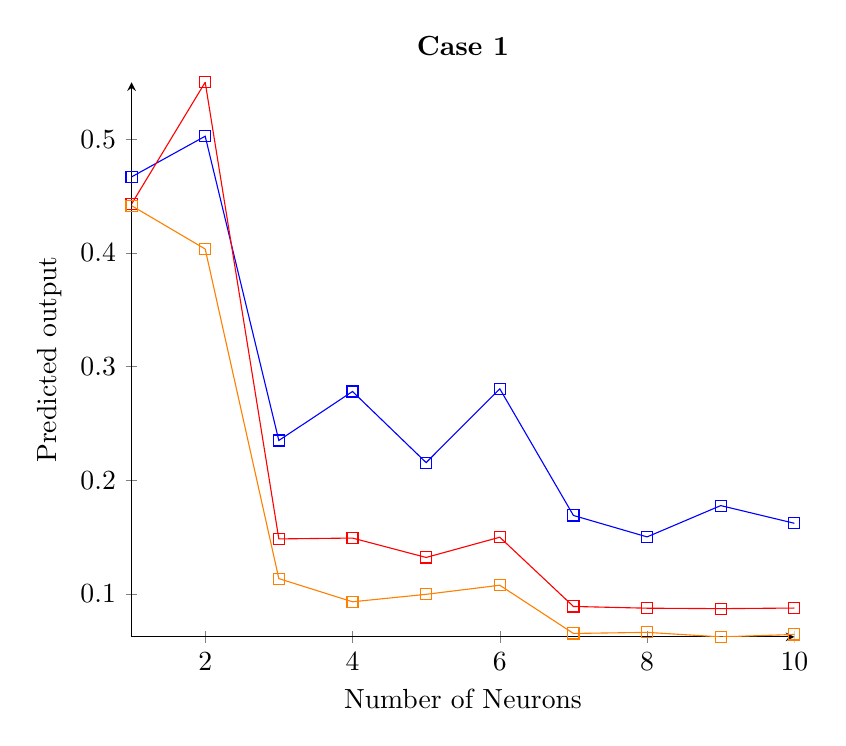
\begin{tikzpicture}

  \begin{axis}[
  title = {\textbf{Case 1}},
  xlabel = { Number of Neurons },
  ylabel = {Predicted output},
  axis lines = left,
  ]

  \addplot[
  color = blue,
  mark = square
  ]coordinates{
  (1, 0.46700647595002565)
  (2, 0.5028392360093282)
  (3, 0.2349874206309317)
  (4, 0.2781089707936994)
  (5, 0.21552533603684487)
  (6, 0.2804885147110787)
  (7, 0.16899363081210655)
  (8, 0.15011050403924103)
  (9, 0.17767823919971779)
  (10, 0.1621070321341431)
  };

  \addplot[
  color = red,
  mark = square
  ]coordinates{
  (1, 0.44312311673152166)
  (2, 0.5503270267577149)
  (3, 0.14834536046098512)
  (4, 0.14910141592641996)
  (5, 0.1320183582461556)
  (6, 0.14984218592549545)
  (7, 0.08888959067283937)
  (8, 0.08735309976544894)
  (9, 0.0869676340911366)
  (10,0.08748945910763019)
  };

  \addplot[
  color = orange,
  mark = square,
  ]coordinates{
  (1, 0.44170244442521933)
  (2, 0.4035404326725686)
  (3, 0.11339664705030737)
  (4, 0.09299640323792795)
  (5, 0.09957419391882207)
  (6, 0.10756599237212054)
  (7, 0.0651219238283709)
  (8, 0.06607782863215868)
  (9, 0.06210818734818407)
  (10, 0.06423135518403288)
  };

  \end{axis}

  \end{tikzpicture}
  \caption{Predicted outputs of Case 1 after 250 training cycles}
  \label{case-1-graph}
\end{figure}

\subsection{Case 2}
\begin{figure}[H]
  \centering
  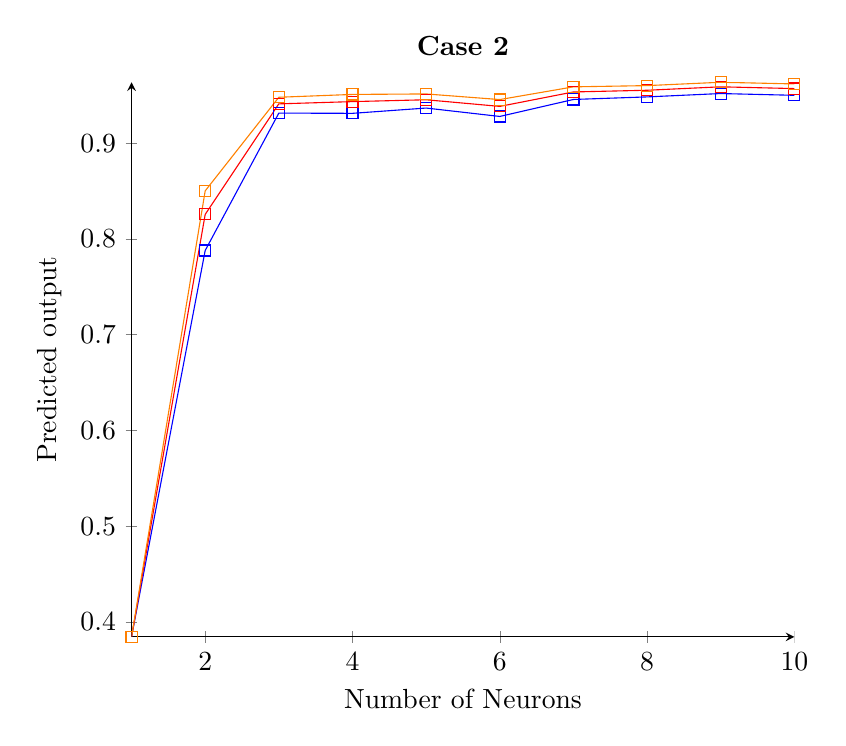
\begin{tikzpicture}
  \begin{axis}[
  title = {\textbf{Case 2}},
  xlabel = { Number of Neurons },
  ylabel = {Predicted output},
  axis lines = left,
  ]

  \addplot[
  color = blue,
  mark = square
  ]coordinates{
  (1, 0.3845247520379267)
  (2, 0.7879033541583771)
  (3, 0.9313644108162242)
  (4, 0.9311129584718981)
  (5, 0.9366281106401981)
  (6, 0.9278541726699097)
  (7, 0.9455892139102183)
  (8, 0.9482674113088276)
  (9, 0.9517773328430301)
  (10, 0.9499330552769415)
  };

  \addplot[
  color = red,
  mark = square,
  ]coordinates{
  (1, 0.38447881868893624)
  (2, 0.8255916212225485)
  (3, 0.9410038577898255)
  (4, 0.9433453569956536)
  (5, 0.9452790420889771)
  (6, 0.9383567074676018)
  (7, 0.9534363449226045)
  (8, 0.9552102575318179)
  (9, 0.9587961079736042)
  (10, 0.9569588093427486)
  };

  \addplot[
  color = orange,
  mark = square,
  ]coordinates{
  (1, 0.3844913722229878)
  (2, 0.8501551206570288)
  (3, 0.9478955606033038)
  (4, 0.9508561620796191)
  (5, 0.9513535139687473)
  (6, 0.9454830990023483)
  (7, 0.958770255998243)
  (8, 0.9600541009733331)
  (9, 0.9635555732608408)
  (10, 0.9618030558596822)
  };

  \end{axis}
  \end{tikzpicture}
  \caption{Predicted outputs of Case 2 after 250 training cycles}
  \label{case-2-graph}
\end{figure}

\subsection{Case 3}
\begin{figure}[H]
  \centering
  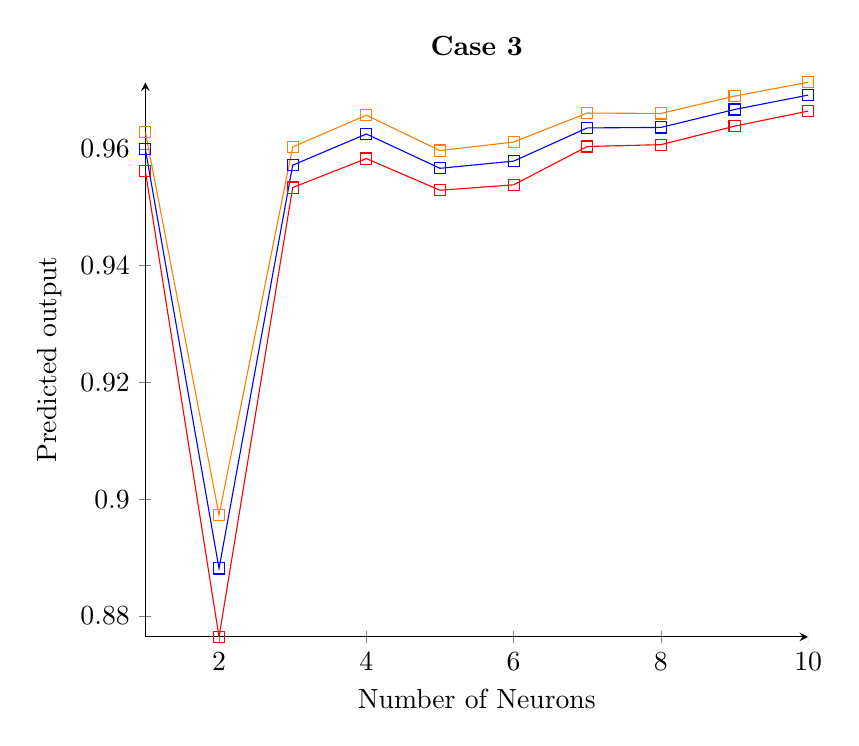
\begin{tikzpicture}
  \begin{axis}[
  title = {\textbf{Case 3}},
  xlabel = { Number of Neurons },
  ylabel = {Predicted output},
  axis lines = left,
  ]

  \addplot[
  color = red,
  mark = square,
  ]coordinates{
  (1, 0.9561878848726166)
  (2, 0.8764339436637559)
  (3, 0.9533906297333611)
  (4, 0.9583528876914469)
  (5, 0.9529310782425574)
  (6, 0.9538579204434591)
  (7, 0.9604225367921141)
  (8, 0.9607327420113712)
  (9, 0.963902514900101)
  (10, 0.9664847853482925)
  };

  \addplot[
  color = blue,
  mark = square,
  ]coordinates{
  (1, 0.9599271359522416)
  (2, 0.8881545826868381)
  (3, 0.9572196803909397)
  (4, 0.9625642388647102)
  (5, 0.9566868538570549)
  (6, 0.9579164705549257)
  (7, 0.9636041927562219)
  (8, 0.9636874159466955)
  (9, 0.9667570555755045)
  (10, 0.9692244623975886)
  };

  \addplot[
  color = orange,
  mark = square,
  ]coordinates{
  (1, 0.9628979718164635)
  (2, 0.897309892973715)
  (3, 0.9603436974794647)
  (4, 0.9657850459026716)
  (5, 0.9597215299885532)
  (6, 0.9611888525661094)
  (7, 0.9661521500152233)
  (8, 0.9660818465663803)
  (9, 0.9690461299728015)
  (10, 0.9714231336912663)
  };

  \end{axis}

  \end{tikzpicture}
  \caption{Predicted outputs of Case 3 after 250 training cycles}
  \label{case-3-graph}
\end{figure}

\subsection{Case 4}
\begin{figure}[H]
  \centering
  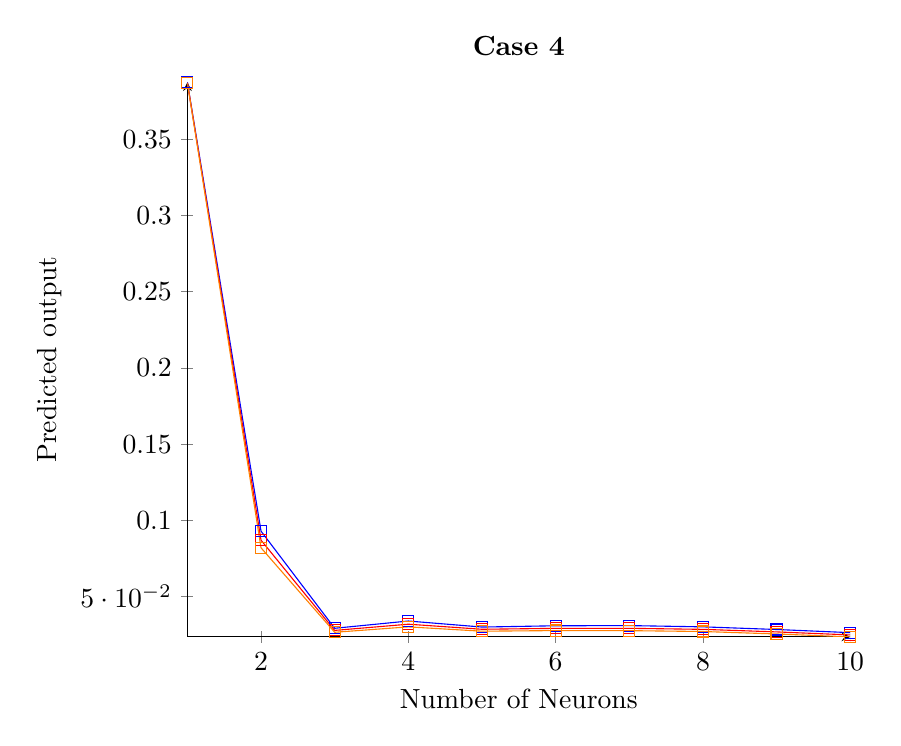
\begin{tikzpicture}
  \begin{axis}[
  title = {\textbf{Case 4}},
  xlabel = { Number of Neurons },
  ylabel = {Predicted output},
  axis lines = left,
  ]

  \addplot[
  color = blue,
  mark = square,
  ]coordinates{
  (1, 0.3873519075938649)
  (2, 0.0929516065383284)
  (3, 0.02925911426093423)
  (4, 0.0340200155781464)
  (5, 0.030062029838706473)
  (6, 0.030904175865449832)
  (7, 0.03102195327771291)
  (8, 0.030196801260093505)
  (9, 0.028462773654088058)
  (10, 0.026393150265471985)
  };

  \addplot[
  color = red,
  mark = square,
  ]coordinates{
  (1, 0.3870978390300801)
  (2, 0.08702526930172703)
  (3, 0.027865367790013293)
  (4, 0.031934535537609166)
  (5, 0.028607899643818716)
  (6, 0.0292055671995101)
  (7, 0.029233053997582466)
  (8, 0.0285557223365103)
  (9, 0.02688023715685751)
  (10, 0.02490011196354535)
  };

  \addplot[
  color = orange,
  mark = square,
  ]coordinates{
  (1, 0.3868915615517505)
  (2, 0.08203553770347201)
  (3, 0.026633002118290745)
  (4, 0.03018269894171098)
  (5, 0.027348018661146577)
  (6, 0.027745567942489734)
  (7, 0.027706580732821832)
  (8, 0.027145187643618805)
  (9, 0.02552686267521916)
  (10, 0.02362238933206421)
  };

  \end{axis}
  \end{tikzpicture}
  \caption{Predicted outputs of Case 4 after 250 training cycles}
  \label{case-4-graph}
\end{figure}

\section{Conclusions and Limitations of This Research }

% God I just want to be done with this thing already
\subsection{Conclusions \label{conclusions}}

As can be seen in figures \ref{case-1-graph}, \ref{case-2-graph}, and \ref{case-4-graph}, at $n = 1$ (such that $n$ is the number of neurons) the neural network produces complete gibberish. It never varies much beyond $Y \approx 0.5$. There is a sharp increase in certainty at $n = 2$ - interestingly, this is also the number of neurons in the input layer. This is not the case in Figure \ref{case-1-graph}, which in two out of three attempts sees a \textit{decrease} in efficiency going from $n = 1$ to $n = 2$. Case 1 is unique in that all input neurons have a value of 0. This may mean that in terms of Big-O Efficiency Notation, Case 1 is the worst possible case. This unique inconsistency in Figure \ref{case-1-graph} may also suggest that the output of the neural network at $n = 2$ is also arbitrary as in the case of $n = 1$, because the input layer in Case 1 is $[0, 0]$ - so the algorithm can't immediately correct itself, since any value $x$ multiplied by $0$ is equal to 0. In all other cases save for Case 3 (which will be explained in more detail further down this section), All neural networks experience a ubiquitous sharp increase in efficiency - indeed, the network only starts to make accurate predictions then - at $n = 2$.

This is likely because the input layer is also two neurons long. At $n = 2$, the number of synaptic weights between the input layer and the intermediary layer is 4 - the same number of the set of possible input/output pairs of an XOR gate. Thus, we can conclude that at $n = 2$, each synaptic link between neurons represents the likelihood of output given a certain set of inputs. This is the minimum number of synaptic weights required for the artificial neural network to function. At $n > 2$, the number of synaptic weights increases exponentially, allowing for more subtle decision-making. This means that the neural network can make more accurate predictions each training cycle.

At $n = 3$, the neural network algorithm again experiences a sharp increase in effeciency, albeit not as sharp of an increase as that at $n = 2$. As shown in Figure \ref{case-1-graph}, The neural network that was least accurate in $n = 2$ - the red one - experienced that greatest correction in accuracy in $n = 3$. This is the Gradient Descent Algorithm (discussed in Section \ref{gradient-descent}) working precisely as intended.

From there, the prediction lines generally slope towards their intended targets, though the algorithm does tend to make errors in the range $4 \leq n \leq 6$. This may validate my hypothesis in Section \ref{objectives}, where I suggested the efficiency of the neural network may be modelled by $O(n log(n))$.

Figure \ref{case-3-graph} is a very bizarre anomaly. At $n = 1$ the neural network's predicted output is very close to the actual output of a logical XOR gate. Then at $n = 2$, the neural network is less accurate than it was at $n = 1$. Furthermore, upon close examination you will notice that the gradient descent algorithm still applies- the further a prediction line is from $Y = 1$ at $n = 1$, the greater the correction was to the algorithm at $n = 2$ - except \textit{it corrected in the wrong direction}. Perhaps the gradient vector had somehow been scaled by a negative factor?

I stated in Section \ref{ANN-definition} that the human programmer can only glimpse how any specific artificial neural network 'thinks', via analyzing the backpropagation algorithm. At higher number of neurons, the artificial neural network has no difficulty correctly guessing the outputs of all four cases of an XOR gate; but this is an intriguing glimpse at its thought process regardless.

\subsection{Limitations}

Using the output of an XOR gate as a training example serves the experiment well in that it is simple . However it carries with it some limitations.

Since an XOR Gate only has two inputs, and $n$ is a set of natural numbers, We can only monitor a neural networks behavior when the intermediary layer is smaller than the input layer for one example: $n = 1$. While it is true that (as explored in Section \label{conclusions}) a neural network only begins to make accurate predictions when the intermediary layer is greater than or equal to the input layer, It would have been beneficial to view if there was a trend in the prediction line if $n$ was smaller than the input layer for several $n$.


\section{Appendix}

\subsection{NeuralNetwork.py \label{neuralnetpy}}

\lstinputlisting[language=Python]{NeuralNetwork.py}
\pagebreak

\subsection{DataCollector.py\label{datacollectorpy}}

\lstinputlisting[language=Python]{DataCollector.py}
\pagebreak

\section{References}

\printbibliography[heading=none]

\end{document}